\chapter{中微子望远镜性能分析}
\label{chap:telescope_performance}

在本章节中,我们研究我们的切伦科夫中微子望远镜对缪子中微子产生的径迹型事件的响应性能。
在模拟和分析研究中,我们以章节\ref{sec:TRIDENT_array}中所介绍的海铃阵列的配置为标准。

\section{角度分辨率}
\label{sec:angular_resolution}

IceCube观测到的弥散中微子流量已经对天体中微子源的参数空间产生了极大的限制:这些源的数量密度必须足够大,而单个源的流强非常微弱。
为了从弥散中微子流量中挖掘出这些微弱的中微子源,下一代的中微子望远镜必须拥有更强的角分辨率\cite{Fang_resolve_flux:2016}。
在本小节中,我们对模拟出来的径迹型中微子事件进行方向重建,通过观察重建的误差来判断海铃的角度分辨率。

中微子望远镜中DOM的大小和分布密度相对于其监控的广袤的海水而言是极其稀疏的。
在一次中微子事件中,大约只有$10^{-7}$的光子信息能够被望远镜中的光敏元件所捕获。
因此,中微子望远镜不是一个量能器,它并不能将粒子所有的能量都沉积其中并且全部测量,相反的,中微子望远镜是一种典型的稀疏采样探测器。
中微子望远镜的重建过程,便是要通过这些有限的光子信息来推断出中微子的动力学信息,即能量,位置和运动方向。

\begin{figure}[!htb]%
    \centering
    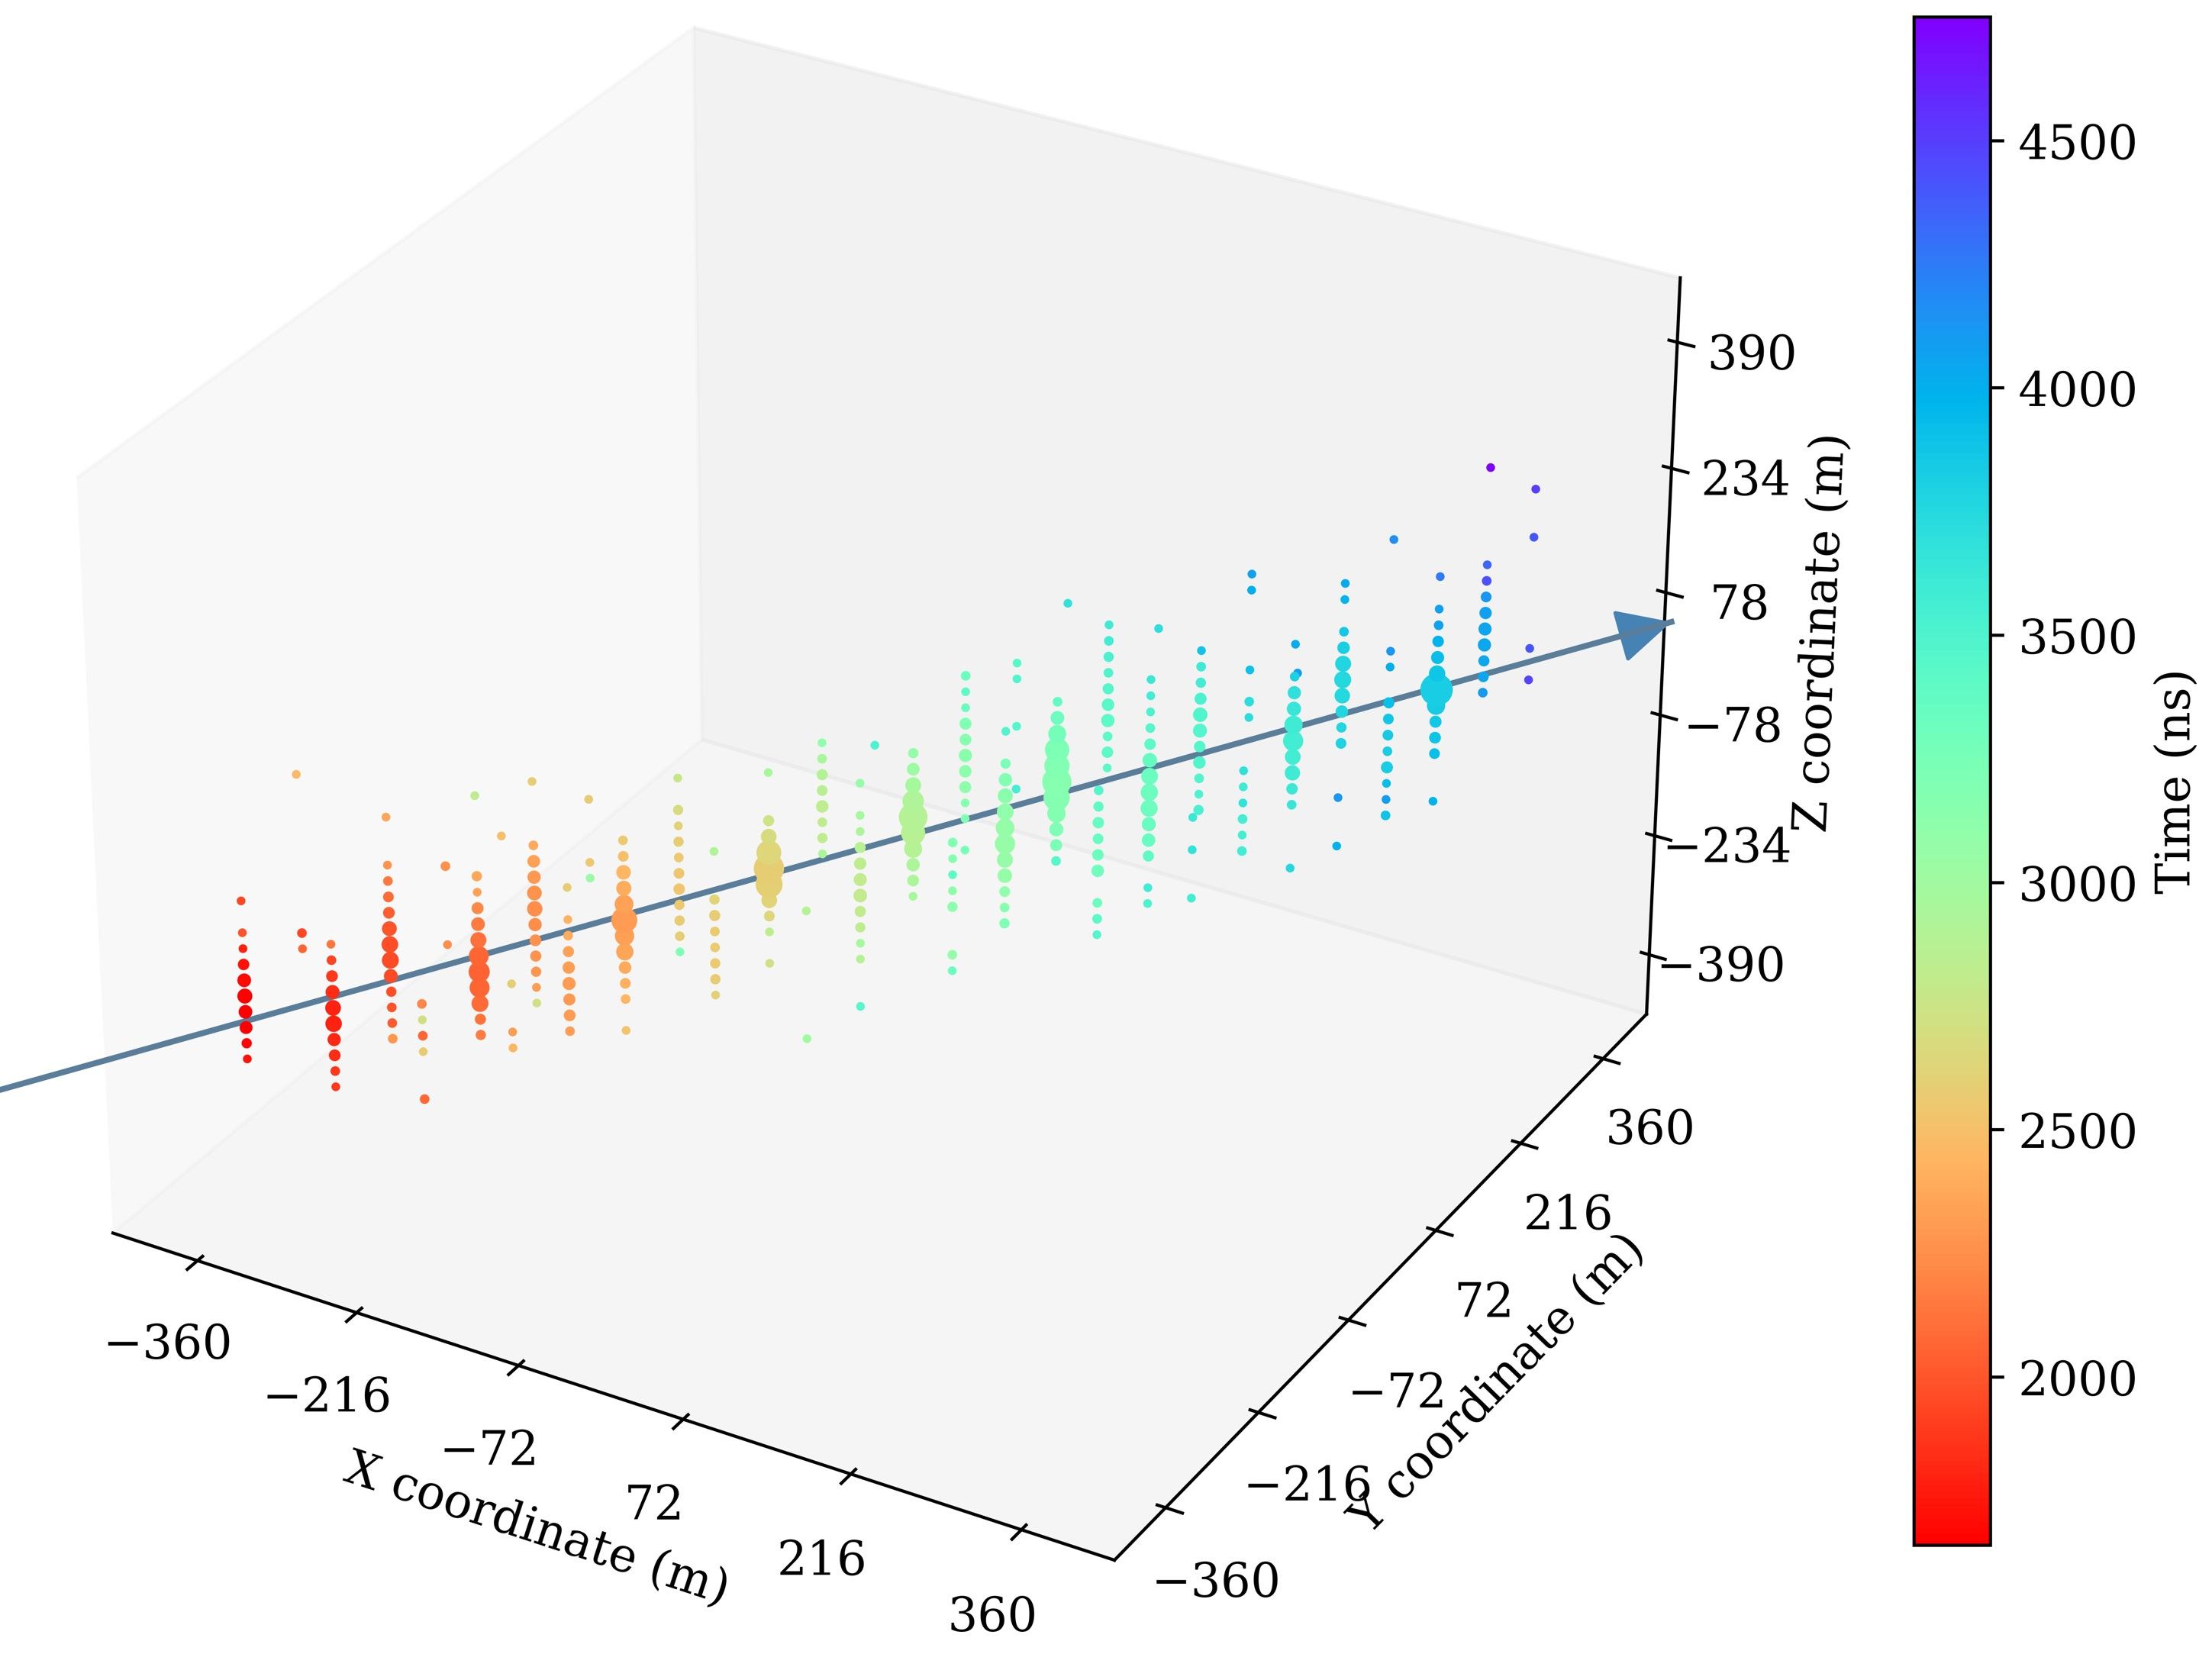
\includegraphics[width=0.75\textwidth]{img/track-like_event.jpg}
    \caption{一个$10\,\mathrm{TeV}$能级的缪子在中微子望远镜中的轨迹。图中的每一个圆点都表示一个接收到光子的hDOM,圆点的大小表示接收到的光子的数量,颜色表示光子到达hDOM的时间。}
    \label{fig:track-like_event}
\end{figure}

一个典型的由缪子产生的径迹型事件在中微子望远镜中留下的轨迹如图\ref{fig:track-like_event}中所示。
从图中我们可以看到,通过阵列中的hDOM的位置与其接收到的光子的时间信息,我们可以看出缪子在阵列中的穿行轨迹。根据这些信息,我们可以对缪子事件进行重建。

\subsection{初步拟合}
\label{subsec:track_reco_first_guess}

对中微子事件的初步拟合是为了针对那些比较低层次,质量杂乱的大量中微子事件,它能够快速确定一个大致的事件方向,也可以用于估计一个事件质量\cite{line_fit:2013, ANTARES_q_fit:2011}。此外,初步拟合得到的方向结果可以作为后续精细拟合的输入参数。

\begin{figure}[!htb]%
    \centering
    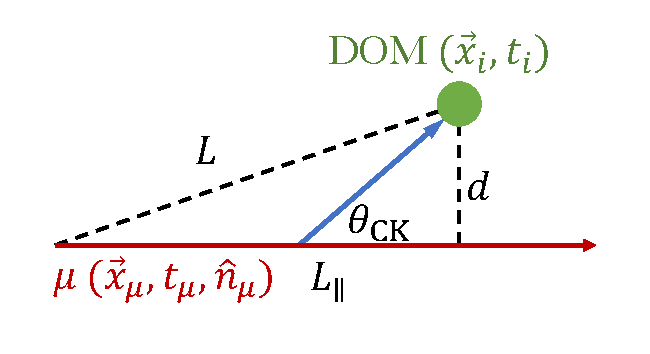
\includegraphics[width=0.75\textwidth]{img/Cherenkov_geometry_DOM_observation.pdf}
    \caption{缪子径迹发射出切伦科夫光子,击中到hDOM上的示意图。}
    \label{fig:Cherenkov_geometry_DOM_observation}
\end{figure}

如图\ref{fig:Cherenkov_geometry_DOM_observation}中所示,假设每一个被光子击中的hDOM的位置和击中时间分别为$\vec{x}_i$和$t_i$,缪子径迹的初始位置,时间和方向分别为$\vec{x}_\mu$,$t_\mu$和$\hat{n}_\mu$。
在初步拟合中,我们首先将缪子产生的切伦科夫光简单地近似成一束与缪子方向平行的平面光,此时hDOM接收的击中信息与初始缪子的运动状态之间应当有如下的近似关系:
\begin{equation}
    t_i \simeq (\vec{x}_i - \vec{x}_\mu) \cdot \hat{n}_\mu + t_\mu ,
\end{equation}
通过对上式进行最小二乘法拟合,我们可以得到对缪子运动信息的初步分析结果。

有了如上的初步结果之后,我们进一步地对缪子的状态进行最大似然估计,在估计中我们所采用的主要观测量为hDOM测量到的光子到达时间的残差$t_i^\mathrm{res}$\cite{AMANDA_track_reco:2003},其定义如下:
\begin{equation}
    t_i^\mathrm{res}(\vec{x}_\mu, t_\mu, \hat{n}_\mu) = t_i - t_i^\mathrm{geo}(\vec{x}_\mu, t_\mu, \hat{n}_\mu),
\end{equation}
其中$t_i^\mathrm{geo}(\vec{x}_\mu, t_\mu, \hat{n}_\mu)$表示在某一径迹假设下,光子到达的几何时间,即切伦科夫光锥面到达该位置的hDOM的时间,根据图\ref{fig:Cherenkov_geometry_DOM_observation}中所示,我们可以写下$t_i^\mathrm{geo}$的表达式:
\begin{equation}
\begin{aligned}
    t_i^\mathrm{geo} &= t_\mu + (L_\parallel - \frac{d}{\tan(\theta_\mathrm{CK})}) / c + \frac{d}{\sin(\theta_\mathrm{CK})} / \frac{c}{n_\mathrm{g}} \\
    &= t_\mu + \frac{L_\parallel}{c} + \frac{d}{c} \times 
    \frac{n_\mathrm{g} n_\mathrm{p} - 1}{\sqrt{n_\mathrm{p}^2 - 1}} \\
    L = \lvert &\vec{x}_i - \vec{x}_\mu \rvert, ~~
    L_\parallel = \lvert (\vec{x}_i - \vec{x}_\mu) \cdot \hat{n}_\mu \rvert, ~~ d = \sqrt{L^2 - L_\parallel^2}
    \label{eq:t_geo}
\end{aligned}
\end{equation}
需要注意的是,介质中的散射效应会导致光子并非沿着直线直接到达hDOM,因此光子的真实到达$t_i$可能会晚于$t_i^\mathrm{geo}$。此外,介质的色散效应以及光敏探测元件自身的时间分辨率会导致观测到的$t_i$也出现一定的弥散。

在处理到达时间时,对于每一个hDOM,我们都只选择出其接收到的第一个光子的到达时间$t_i^\mathrm{1st}$而忽略其余剩下的光子的到达时间,这是因为第一个到达的光子更有可能是没有经过任何散射而直接到达hDOM的。
并且考虑到SiPM的时间分辨性能要高于PMT,在一个hDOM中的PMT和SiPM都同时有信号的情况下,我们优先采用SiPM中测量到的时间。

我们首先构建一个形式上最为简洁,并且计算效率和稳定性都非常良好的最大似然函数$\mathcal{L}^M$,我们称之为M-estimator:
\begin{equation}
    \ln \mathcal{L}^M(\vec{x}_\mu, t_\mu, \hat{n}_\mu; \vec{x}_i, t_i^\mathrm{1st}) = 
    \sum_i \left(2 - 2 \sqrt{ (t_i^\mathrm{res})^2/2 + 1 } \right) .
\end{equation}
这样构造出来的似然函数在数学上是一个凸函数,因此能够很快得收敛到全局最优解。
然而$\mathcal{L}^M$中的$t_i^\mathrm{res}$的概率分布函数并非是真正物理上的分布函数。

\subsection{光子到达时间分布函数}

由于光子的行为在经过多次散射之后就变得难以估计,因此我们依赖于使用数值模拟的方法,从大量的模拟得到的$t^\mathrm{res}$中去估计出它的分布函数。
我们模拟得到的$t^\mathrm{res}$如图\ref{fig:residual_time_distribution}中所示。
我们将$t^\mathrm{res}$表示为一个与hDOM的位置到径迹的距离$d$相关的函数$t^\mathrm{res}(d)$,这是考虑到它们之间的距离决定了光子从发射到被接收时中间走过的距离,而这正决定了光子经历的散射次数。

为拟合模拟中得到的分布,我们采用了如下形式的函数来表示$t^\mathrm{res}$的分布:
\begin{equation}
    p(\tau) = \frac{1}{\pi (\tau^2+1)} \times \frac{2}{e^{-\alpha \tau} + 1} ,
    \label{eq:residual_time_PDF}
\end{equation}
其中,$\tau = (t_\mathrm{res} - \mu) / \sigma$是经过平移并且无量纲化之后的到达时间残差,$\alpha$表示分布的倾斜程度。
式\ref{eq:residual_time_PDF}中的第一项表示一个柯西分布,它被用于描述到达时间的不确定性;而第二项是一个sigmoid函数,它使得原本沿着$y$轴对称的柯西分布向右侧倾斜,从而可以表示散射光子到达时间的延后。
式\ref{eq:residual_time_PDF}很好地展现出在海水中,大部分的光子都可以直接到达探测器,进而在$t_\mathrm{res} = 0\,\mathrm{ns}$的位置形成一个峰,而少部分光子则会延后到达。
此外,相比于过去其他实验所使用的伽马分布\cite{AMANDA_track_reco:2003},公式\ref{eq:residual_time_PDF}在$t_\mathrm{res} < 0$的区域也是良好定义的,可以表现出由于光子色散和探测器的事件响应精度问题而导致光子先于几何时间到达探测器,并且在数值求解的过程中也有较好的稳定性。

我们将公式中的形状参数$\mu$,$\sigma$和$\alpha$表示为有关hDOM到径迹的距离$d$的一次函数,对模拟得到的数据点进行拟合,其得到的结果如下:
\begin{equation}
    \mu = 0.0199 d - 0.114,~~
    \sigma = 0.0669 d + 0.328,~~
    \alpha = 0.0127 d + 0.538 ,
    \label{eq:residual_time_parameters}
\end{equation}
我们在拟合的过程中只采用了光子到达时间位于2.5\%到70.5\%之间的数据,因为这部分光子是最有可能成为第一个到达的光子。拟合结果与实验模拟数据之间的比较如图\ref{fig:residual_time_distribution}中所示。

\begin{figure}[!htb]%
    \centering
    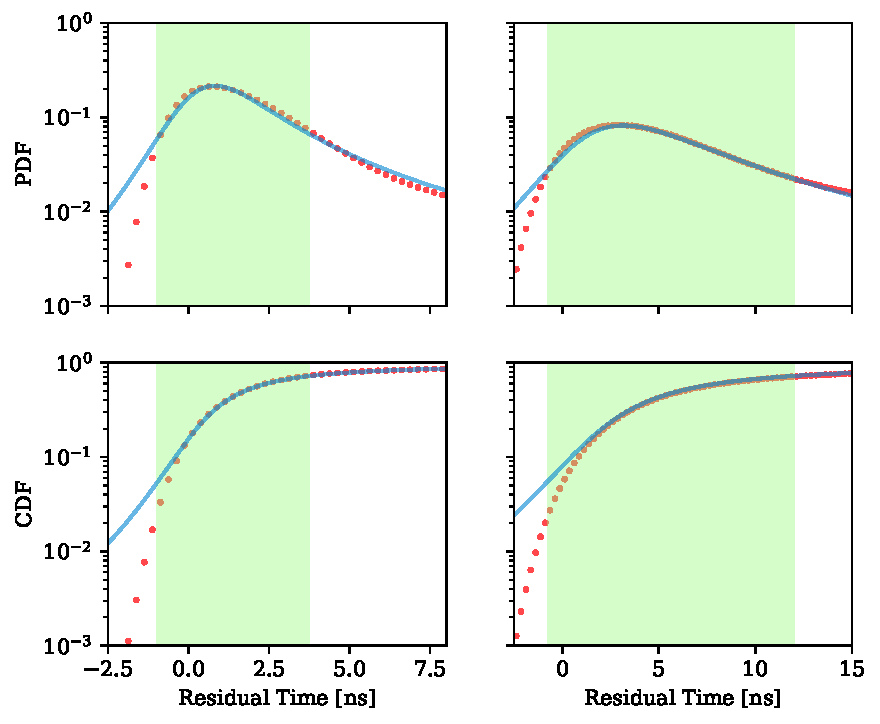
\includegraphics[width=0.85\textwidth]{img/residual_time_distribution.pdf}
    \caption{模拟得到的光子到达时间残差$t^\mathrm{res}$的分布以及解析拟合。左图为hDOM到径迹距离$d = 20 \,\mathrm{m}$下的分布,右图为$d = 70 \,\mathrm{m}$下的分布。上图为概率密度分布函数,而下图为累积分布函数。图中绿色的阴影区域表示累积分布函数的值为2.5\%和70.5\%的区域范围,只有在这个范围内的概率分布函数数据点才被用于拟合解析表达式。}
    \label{fig:residual_time_distribution}
\end{figure}

有了更为准确的光子到达时间表示之后,我们可以将构造更为精细的似然函数:
\begin{equation}
    \mathcal{L}(\vec{x}_\mu, t_\mu, \hat{n}_\mu; \vec{x}_i, t_i^\mathrm{1st}) = 
    \prod_i \left( \frac{1}{\pi (\tau^2+1)} \times \frac{2}{e^{-\alpha \tau} + 1} \right),
    \label{eq:track_reco_likelihood}
\end{equation}
将上一节中的初步重建结果作为初始条件代入到优化算法中,我们可以寻找使得\ref{eq:track_reco_likelihood}达到最大值的径迹方向。


\subsection{重建结果}

对不同入射能量缪子中微子产生的径迹型事件,我们的重建结果如图\ref{fig:angular_resolsution}中所示。
我们可以看到我们的重建算法对能量仅为$1\,\mathrm{TeV}$的中微子事件也可以达到$\sim 0.3^\circ$的重建精度,但此时中微子和缪子在反应顶点处的本征方向误差占据主导地位,因此望远镜对真实中微子的角分辨率处于$\lesssim 1^\circ$的水平。
而在$100\,\mathrm{TeV}$到$1\,\mathrm{PeV}$的能量范围内,探测器的角分辨率可以达到$\sim 0.1^\circ$的量级,达到了世界最顶尖的角分辨率水平。
如此优越的性能与探测器中采用的SiPM光敏元件的高时间分辨率有直接的关系,有关此内容的讨论参见章节\ref{sec:hdom}。


\begin{figure}[!htb]%
    \centering
    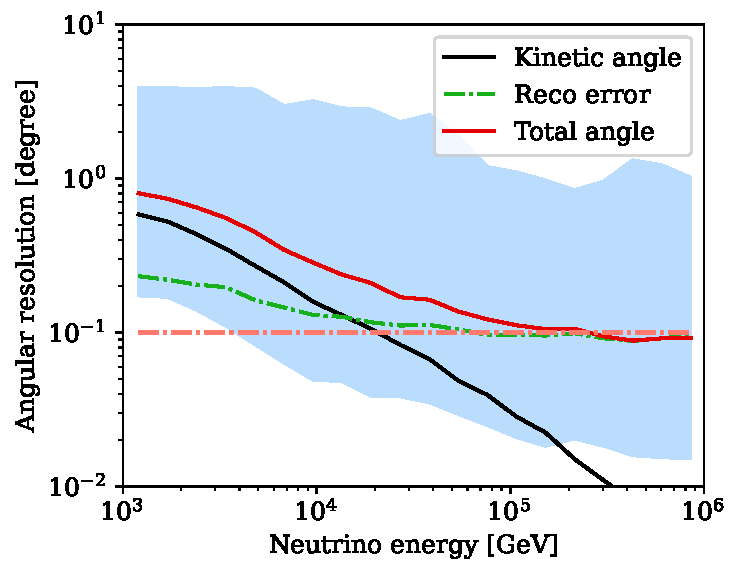
\includegraphics[width=0.75\textwidth]{img/angular_resolsution.pdf}
    \caption{对不同的缪子中微子产生的径迹型事件进行重建后,得到的中微子望远镜的角分辨率。图中绿色点虚线表示对缪子径迹的重建误差,黑色实线表示中微子与DIS反应得到的缪子之间的动能夹角,红色实线表示重建得到的径迹方向与真实中微子方向之间的误差,这三条线均表示角度误差的中位数。蓝色阴影带状区域表示重建得到的径迹方向与真实中微子方向之间的误差的$1\sigma$分布区域。}
    \label{fig:angular_resolsution}
\end{figure}



\section{有效面积}

在本节中,我们研究海铃中微子望远镜对缪子径迹型事件的有效面积。探测器的有效面积$A_\mathrm{eff}$是衡量探测器能够探测到的事例率的重要性能指标。
假设中微子的物理流量为$F_\mathrm{phy}(\hat{n}, E)$,探测器的有效面积被定义为:
\begin{equation}
    A_\mathrm{eff} (\hat{n}, E) \equiv \frac{\mathrm{d}N}{\mathrm{d}t \,\mathrm{d}\Omega \,\mathrm{d}E} (\hat{n}, E) / 
    F_\mathrm{phy}(\hat{n}, E) ,
    \label{eq:eff_area_init}
\end{equation}
其中$\frac{\mathrm{d}N}{\mathrm{d}t \,\mathrm{d}\Omega \,\mathrm{d}E}(E, \hat{n})$表示在某一能量$E$和方向$\hat{n}$上,单位时间单位能量单位立体角上,探测器所能观测到的事件数量。

在后面的分析计算中,我们将会看到探测器的有效面积与具体的中微子辐射源无关,其反应的是探测器的本质性能。
尽管如此,我们通常借助于一些假定的中微子源,通过蒙特卡洛采样的方法研究探测器对不同中微子事件的响应,进而分析出探测器的有效面积。


\subsection{采样权重}
\label{subsec:weightings}

考虑真实的物理情况,对于任意的中微子流强$F_\mathrm{phy}(E, \hat{n})$而言,在单位能量单位时间单位空间单位立体角内,中微子在某一个点上发生DIS过程的数量是:
\begin{equation}
\begin{aligned}
    \frac{\mathrm{d}N}{\mathrm{d}E ~\mathrm{d}\Omega ~\mathrm{d}t ~\mathrm{d}V} (E, \hat{n}, \vec{x})
    &= F_\mathrm{phy}^\mathrm{surv} (\hat{n}, E, X)\times \frac{1}{\lambda_\mathrm{int}(E)} \\
    &= F_\mathrm{phy}(\hat{n}, E) \times P_\mathrm{surv}(E, X) \times \frac{1}{\lambda_\mathrm{int}(E)} , \\
    P_\mathrm{surv}(E, X) = e&^{- \frac{\sigma_\mathrm{tot}(E) \times X(\hat{n}, \vec{x})}{m_{p}}}, ~~~
    X(\hat{n}, \vec{x}) = \int_l \rho(\vec{x'}) \,\mathrm{d}\vec{x'}, ~~~
    \lambda_\mathrm{int}(E) = \frac{m_{p}}{\rho(\vec{x}) \sigma_\mathrm{DIS}(E)}
\end{aligned}
\label{eq:sampling_phy_pdf}
\end{equation}
其中$E$,$\hat{n}$和$\vec{x}$分别表示中微子的能量,方向和位置。
$F_\mathrm{phy}^\mathrm{surv} (\hat{n}, E, X)$表示在地球中穿过柱密度$X$之后,能够存活下来的中微子的流强。
$P_\mathrm{surv}(E, X)$表示存活概率,$\sigma_\mathrm{tot}(E)$表示中微子与物质相互作用的总散射截面,柱密度$X(\hat{n}, \vec{x})$与中微子在地球中的路径以及地球的密度模型有关。
$\lambda_\mathrm{int}(E)$表示中微子的反应自由程,$m_p$表示质子质量\footnote{这里我们忽略了质子与中子之间散射截面与质量的差异,而用同位旋为0的核子来表示散射截面,用$m_p$来表示质子和中子的平均质量。}
$\rho(\vec{x})$表示介质的密度,与地球的密度模型有关,$\sigma_\mathrm{DIS}(E)$表示感兴趣的DIS反应通道的散射截面。

以一个具体的问题为例,假设我们要研究探测器能探测到的中微子事例率,那么我们可以通过如下表达式来计算实例率:
\begin{equation}
    \frac{\mathrm{d}N}{\mathrm{d}t} = 
    \int \mathrm{I}_\mathrm{sel}(s) \times \frac{\mathrm{d}N}{\mathrm{d}E ~\mathrm{d}\Omega ~\mathrm{d}t ~\mathrm{d}V} 
    ~\mathrm{d}E ~\mathrm{d}\hat{n} ~\mathrm{d}\vec{x} ,
    \label{eq:sampling_phy_trigger}
\end{equation}
其中我们引入了符号$s$(signal)来表示由能量$E$,方向$\hat{n}$的中微子在位置$\vec{x}$发生DIS过程引起的探测器探测到的信号。严格来说$s$是一个分布,因为粒子的相互作用结果是不确定的,同样的中微子所引发的事件会产生不同的信号,这种不确定性可以通过大量的模拟采样来消除。
$\mathrm{I}_\mathrm{sel}(s)$表示事件筛选算法对事件$s$的响应结果,它根据信号的强弱程度,质量高低,以及与分析目标的符合程度返还1或者0的值。

在我们的重要性采样的过程中,我们使用蒙特卡洛采样的方式来代替积分,即我们将积分运算理解为了对物理量求期望。
蒙特卡洛采样中注入的模拟事件在相空间中的具体分布是可以由我们自己设计的,通常我们会将之与感兴趣的物理研究对象联系在一起,例如侧重于某一中微子的能量和入射角区间。
假如我们采用了如下的能量,方向和位置的分布函数:
\begin{equation}
    P_\mathrm{mc} (E, \hat{n}, \vec{x}) = F_\mathrm{mc} (E, \hat{n}) \times n_\mathrm{mc}(\vec{x}) ,
    \label{eq:sampling_MC_pdf}
\end{equation}
其中$F_\mathrm{mc} (E, \hat{n})$是我们想要研究并且在模拟中注入的中微子能谱,有$E^{-1} \Omega^{-1}$的量纲,$n_\mathrm{mc}(\vec{x})$是注入的中微子反应事件的顶点在空间上的分布函数,有$V^{-1}$的量纲。
在真实物理世界中,中微子流强的能谱指数$\alpha_\mathrm{phy}$通常为$-2$到$-3$,在这种情况下,探测器探测到的信号绝大多数都是低能的无法通过质量筛选的信号,对这些低能信号做模拟将会浪费大量的计算资源。
而在重要性采样中,我们可以将能谱指数$\alpha_\mathrm{mc}$设计成$-1$到$-1.5$,以此来产生更多的我们感兴趣高能的事件。

我们将我们的蒙特卡洛采样的分布函数插入到式\ref{eq:sampling_phy_trigger}中,可以得到:
\begin{equation}
\begin{aligned}
    \frac{\mathrm{d}N}{\mathrm{d}t} &= 
    \int \mathrm{I}_\mathrm{sel}(s) \times 
    \frac{\mathrm{d}N}{\mathrm{d}E ~\mathrm{d}\Omega ~\mathrm{d}t ~\mathrm{d}V}(E, \hat{n}, \vec{x}) 
    ~\mathrm{d}E ~\mathrm{d}\hat{n} ~\mathrm{d}\vec{x} \\
    &= \int \mathrm{I}_\mathrm{sel}(s) \times 
    \frac{\mathrm{d}N}{\mathrm{d}E ~\mathrm{d}\Omega ~\mathrm{d}t ~\mathrm{d}V} (E, \hat{n}, \vec{x})
    \times \frac{1}{P_\mathrm{mc} (E, \hat{n}, \vec{x})} \times P_\mathrm{mc} (E, \hat{n}, \vec{x})
    ~\mathrm{d}E ~\mathrm{d}\hat{n} ~\mathrm{d}\vec{x} \\
    &= \mathbb{E}_s \left[ \mathrm{I}_\mathrm{sel}(s) \times 
    \frac{\mathrm{d}N}{\mathrm{d}E ~\mathrm{d}\Omega ~\mathrm{d}t ~\mathrm{d}V} (E, \hat{n}, \vec{x})
    \times \frac{1}{F_\mathrm{mc} (E, \hat{n}) \times n_\mathrm{mc}(\vec{x})}   \right]  \\
    &= \frac{1}{N_\mathrm{tot}} \sum^N_i \left[ 
    \mathrm{I}_\mathrm{sel}(s_i) \times 
    \frac{\mathrm{d}N}{\mathrm{d}E ~\mathrm{d}\Omega ~\mathrm{d}t ~\mathrm{d}V} (E_i, \hat{n}_i, \vec{x}_i)
    \times \frac{1}{F_\mathrm{mc} (E_i, \hat{n}_i) \times n_\mathrm{mc}(\vec{x}_i)} \right]
\end{aligned}
\label{eq:sampling_MC_trigger}
\end{equation}
在最后一步中,我们用蒙特卡洛采样的方式代替了期望计算。其中$s_i$表示某一个根据$P_\mathrm{mc} (E, \hat{n}, \vec{x})$分布采样得到的模拟事件样本,$N_\mathrm{tot}$表示采样样本总数。

进一步的,我们将中微子发生反应的表达式(\ref{eq:sampling_phy_pdf})带入到事例率的表达式(\ref{eq:sampling_MC_trigger})中,并且将结果拆解成更加模块化的组分:
\begin{equation}
\begin{aligned}
    \frac{\mathrm{d}N}{\mathrm{d}t} 
    &= \frac{1}{N_\mathrm{tot}} \sum^N_i \left[ \mathrm{I}_\mathrm{sel}(s_i) \times 
    \frac{\mathrm{d}N}{\mathrm{d}E ~\mathrm{d}\Omega ~\mathrm{d}t ~\mathrm{d}V} (E_i, \hat{n}_i, \vec{x}_i)
    \times \frac{1}{F_\mathrm{mc} (E_i, \hat{n}_i) \times n_\mathrm{mc}(\vec{x}_i)} \right] \\
    &= \frac{1}{N_\mathrm{tot}} \sum^N_i \left[ \mathrm{I}_\mathrm{sel}(s_i) \times 
    F_\mathrm{phy}(E_i, \hat{n}_i) \times
    P_\mathrm{surv}(E_i, X_i) \times
    \frac{1}{\lambda_\mathrm{int}(E_i)} \times
    \frac{1}{F_\mathrm{mc} (E_i, \hat{n}_i)} \times
    \frac{1}{n_\mathrm{mc}(\vec{x}_i)} \right]
\end{aligned}
\label{eq:sampling_MC_terms_trigger}
\end{equation}

在上述表达式中,$\mathrm{I}_\mathrm{sel}(s)$依赖于探测器的探测能力以及对事件的筛选方式,中微子的物理流量$F_\mathrm{phy}(E, \hat{n})$对应于具体的某一个中微子源的测量结果或者对源流量的假设,$\lambda_\mathrm{int}(E)$与$P_\mathrm{surv}(E, X)$与中微子与物质的散射截面以及地球模型相关,$F_\mathrm{mc} (E, \hat{n})$和$n_\mathrm{mc}(\vec{x})$与采样的方式有关。在实际应用中,我们将后面四项作为权重项:
\begin{equation}
\begin{aligned}
    w_\mathrm{tot} &= w_\mathrm{surv} \times w_\mathrm{int} \times w_\mathrm{flux} \times w_\mathrm{vol} \\
    w_\mathrm{surv} &= P_\mathrm{surv}(E, X), &\mathrm{dim}(1) \\
    w_\mathrm{int} &= \frac{1}{\lambda_\mathrm{int}(E)}, &\mathrm{dim}(L^{-1}) \\
    w_\mathrm{flux} &= \frac{1}{F_\mathrm{mc}(E, \hat{n})},  &\mathrm{dim}(E \Omega) \\
    w_\mathrm{vol} &= \frac{1}{n_\mathrm{mc}(x_i)} = V_\mathrm{sample}, &\mathrm{dim}(L^{3}) ,\\
\end{aligned}
\label{eq:weighting_terms}
\end{equation}
其中$w_\mathrm{tot}$表示总的权重大小。将其带回式子\ref{eq:sampling_MC_terms_trigger}中可以得到:
\begin{equation}
    \frac{\mathrm{d}N}{\mathrm{d}t} = 
    \frac{1}{N_\mathrm{tot}} \sum^N_i \left[ 
    \mathrm{I}_\mathrm{sel}(s_i) \times 
    F_\mathrm{phy} (E_i, \hat{n}_i) \times
    w_{\mathrm{tot}, i} \right]
\label{eq:sampling_trigger_rate}
\end{equation}

公式\ref{eq:weighting_terms}中的$V_\mathrm{sample}$表示采样的体积,在章节\ref{subsec:muon_sampling}中所描述的针对径迹型缪子中微子事件的采样模式下,我们的采样体积为:
\begin{equation}
    V_\mathrm{sample}^\mathrm{track} = \pi R_0^2 (D_\mu + 2D_0) ,
    \label{eq:weighting_volume}
\end{equation}
而对于普通的非径迹型中微子事件,只有当DIS反应的顶点位置发生在望远镜阵列的内部时,事件才可以被探测到,因此采样体积即为探测器的几何体积:
\begin{equation}
    V_\mathrm{sample}^\mathrm{non-track} = V_\mathrm{det} ,
    \label{eq:weighting_volume_2}
\end{equation}

\subsection{事件筛选方法}

\begin{figure}[!htb]%
    \centering
    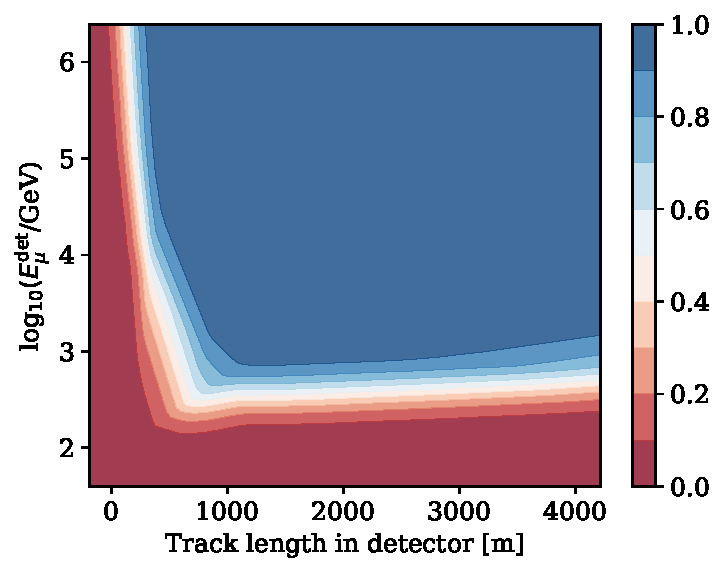
\includegraphics[width=0.75\textwidth]{img/trigger_rate_nn.pdf}
    \caption{缪子径迹型事件的筛选通过几率与缪子能量$E_\mu^\mathrm{det}$以及缪子在探测器内的穿行长度$L_\mu$的关系。}
    \label{fig:trigger_rate_nn}
\end{figure}

为中微子望远镜设计事件筛选算法是为了在存在高噪声的环境中筛选出像是有价值的信号\cite{KM3NeT_trigger:ICRC2019, IceCube_trigger:2015, KM3NeT_trigger:2018}。
在深海中运行的中微子望远镜会受到多种不同的噪声的影响:PMT的暗噪声($\lesssim 1 \,\mathrm{kHz} / \mathrm{PMT}$),海水的K40放射性衰变产生的切伦科夫光($\sim 2 \,\mathrm{kHz} / \mathrm{PMT}$)\cite{KM3NeT_K40:2017},有机物在受到扰动后激发出的光信号,深海鱼类发出的生物光信号\cite{ANTARES_biolumi:2021, Baikal_biolumi:2021}等等。

目前关于海铃探测器的研究尚处于早期阶段,我们对噪声对中微子信号分析的影响尚未完全考虑清楚。因此在以下的研究中,我们主要考虑一些信号强度比较高,不容易受到噪声影响的径迹型事件。我们在以下分析中将事件筛选的标准设置为:
\begin{enumerate}
    \item 事件中PMT探测到的NPE数量大于15。
    \item 经过重建算法后,重建得到的方向与真实中微子的方向之间的误差小于6度。
\end{enumerate}

通过模拟大量的缪子径迹型事件数据并对他们施加设计的事件筛选标准,再使用一个多层感知器来拟合筛选结果,我们可以通过训练得到通过筛选的几率与到达探测器的缪子能量$E_\mu^\mathrm{det}$以及缪子在探测器内的穿行长度$L_\mu$的关系如图\ref{fig:trigger_rate_nn}所示。


\subsection{对模拟事件的统计分析}

通过在探测器中注入大量的模拟事例,我们可以进行一些统计分析来检验事件产生器模拟程序的结果,同时,这也能加深对中微子望远镜探测到的事件分布的理解。
我们在$1\,\mathrm{TeV} - 10\,\mathrm{PeV}$的能量范围内,以谱指数为$-1.1$的能谱注入了400k个缪子中微子带电流事件。其中,有156k个事件中的缪子能够顺利到达探测器,而其他缪子或是因为中途就被介质所吸收,或是因为注入时没有对准探测器,导致没能在探测器中产生有效的信号。因此,在这一批次的模拟中,我们的事件产生器的命中率,或者说采样效率约为$40\%$。

图\ref{fig:sampling_energy_spectrum_unweighted}展示了在这一批模拟注入的事件中成功到达探测器的事件的初始中微子能量的分布。
可以看到我们在产生器中设置的$-1.1$的注入能谱使得在各个中微子能量范围内都有充足的事件分布。
同时我们也可以发现向下运动的中微子事件比向上运动的中微子事件在数量上要更多一些,这是因为向下注入时,海水的厚度和密度都比较小,缪子的能损程度较少,因此缪子有更大的几率能到达探测器。

\begin{figure}[!ht]%
    \centering
    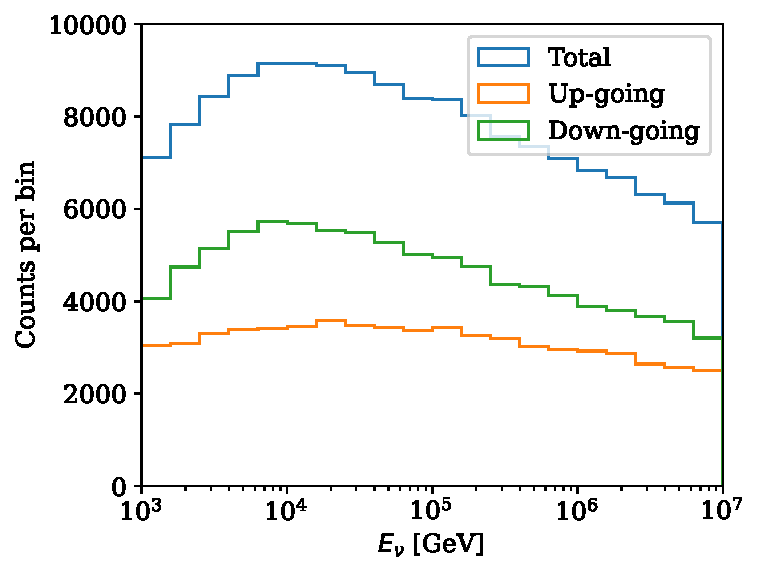
\includegraphics[width=0.72\textwidth]{img/sampling_energy_spectrum_unweighted.pdf}
    \caption{模拟中成功注入的事件在中微子的能量和入射方向上的分布。}
    \label{fig:sampling_energy_spectrum_unweighted}
\end{figure}

\begin{figure}[!ht]%
    \centering
    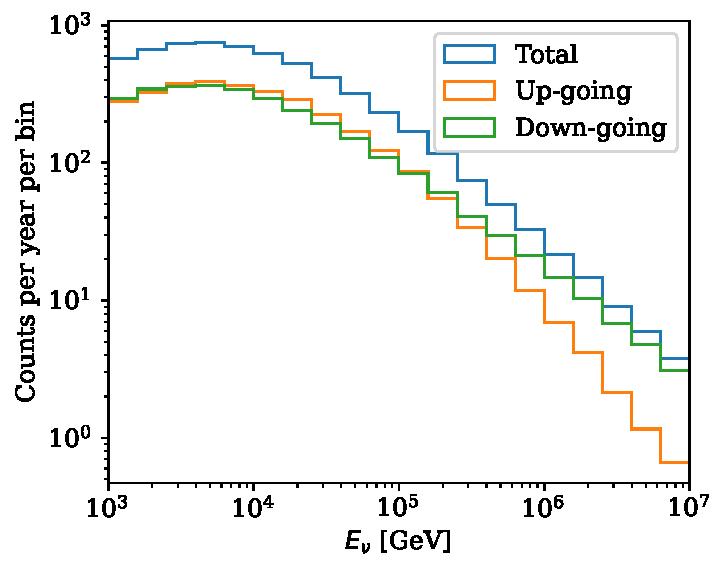
\includegraphics[width=0.72\textwidth]{img/sampling_energy_spectrum.pdf}
    \caption{对于弥散的天体物理中微子流,在经过加权处理后,探测器在不同中微子的能量和入射方向上的事例率。}
    \label{fig:sampling_energy_spectrum}
\end{figure}

为了对探测器进行有物理意义的分析,我们需要把注入的事件与权重项$w_\mathrm{tot}$结合起来分析,同时我们还需要假设一个分析的物理能谱。
在本小节中,我们将研究对象定为弥散的全天各向同性的缪子中微子能谱,即我们将公式\ref{eq:diffse_nu_flux}中的谱指数和流强取为-2.35和1.45\cite{IceCube_diffse_muon:2021}。

图\ref{fig:sampling_energy_spectrum}中显示了在添加权重之后,探测器对不同的入射能量和方向的中微子的事例率。我们可以发现,随着中微子能量逐渐升高,探测到的事例率先上升后逐渐减少,在能量超过$10\,\mathrm{TeV}$后,它们的关系大致呈:
\begin{equation}
    \frac{\mathrm{d}N}{\mathrm{d}t\mathrm{d}E} \propto E_\nu^{-1.7}, 
    \label{eq:diffse_nu_mu_flux_observed}
\end{equation}
其中$\frac{\mathrm{d}N}{\mathrm{d}t\mathrm{d}E}$表示时间单位能量下探测器观测到的弥散缪子中微子流的事例率。


同时,我们也可以看到在经过加权后能够反映物理真实的事件分布中,在能量比较低时($E_\nu \lesssim 0.1\,\mathrm{PeV}$),入射方向向上的中微子的事例率与入射方向向下的事例率几乎没有差别。
而能量比较高($E_\nu > 1\,\mathrm{PeV}$)的情况下,入射方向向上的中微子事件比入射方向向下的中微子事件在事例率要小约2到10倍。
这种上下方向事件数的不对称是由一些几何效应引起的,几何效应主要包括两方面:宏观上地球的几何以及探测器附近的几何。

宏观上地球的几何导致向上和向下的中微子事件穿透地球的概率不同。随着能量的升高,中微子与物质的相互作用截面增大,地球的吸收作用使得大量向上运动的中微子在穿越地球的过程中就已经发生了反应。
不同能量不同入射角的中微子事件穿透地球的概率如图\ref{fig:survival_probability}所示。
从图中我们可以看到,能量大于$1\,\mathrm{PeV}$的中微子只有$\lesssim 0.1$的概率能够穿透地球。图中$\cos(\theta_z)=-0.85$处穿透率的突然变化是由于地球密度变化导致的,此入射角对应于中微子是否穿过密度最高的地核的分界线。


\begin{figure}[!htb]%
    \centering
    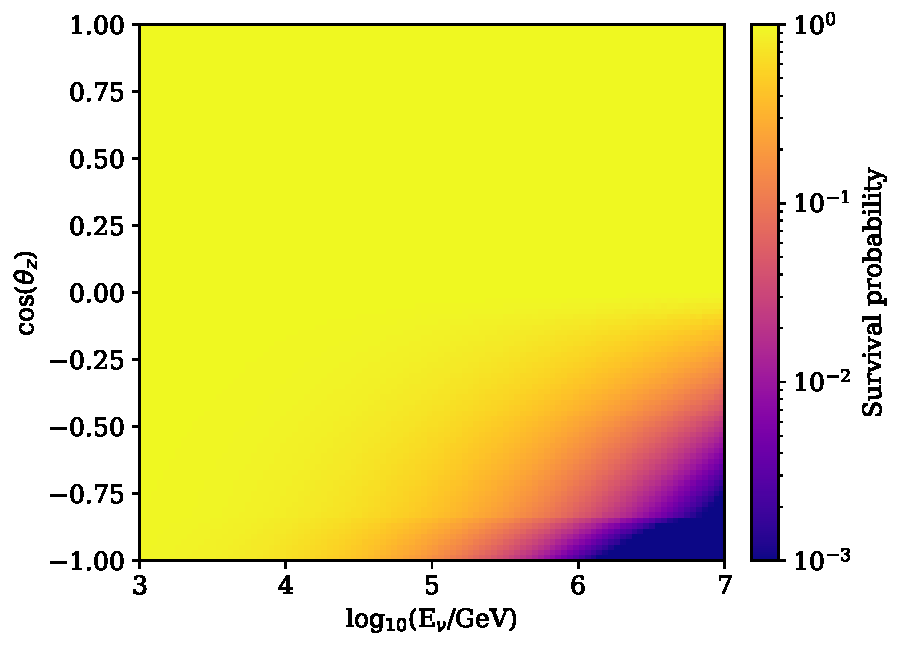
\includegraphics[width=0.75\textwidth]{img/survival_probability.pdf}
    \caption{不同能量$E_\nu$和不同天顶角$\theta_z$的中微子能够成功穿越地球的概率。}
    \label{fig:survival_probability}
\end{figure}

探测器附近几何结构的影响是指在缪子径迹的长度范围内(对于海水而言约$\sim 10\,\mathrm{km}$),介质密度的变化。在模拟中,我们将中微子望远镜阵列的中心放置在水下$2900\,\mathrm{m}$处,因此沿望远镜中心向上$2900\,\mathrm{m}$即到达了海水和空气的交界面,向下$500\,\mathrm{m}$便是海水和岩石的交界面。
如图\ref{fig:sampling_dis_position}所示,向上的缪子中微子事件可以来自地壳深处约$4\,\mathrm{km}$处,而向下的缪子事件由于受到水深的限制,最多只能来自于$2900\,\mathrm{m}$外的海水中,因此向上的事件可供中微子发生DIS反应的靶物质质量要大于向下的事件。
然而虽然向上的事件拥有更大的可反应物质量,但其产生的缪子在介质中穿行时会损失更大的能量。
在图\ref{fig:sampling_energy_spectrum_det}中,我们观察到在选取了高能($E_\nu > 1\,\mathrm{PeV}$)的中微子事件之后,向下运动的中微子事件通常拥有更高的到达探测器的能量,而向上运动的中微子事件在到达探测器的能量上更加的弥散。这种效应会导致向上运动的中微子事件对原初中微子的能量重建的效果较差,因为我们难以知道缪子究竟在探测器外损失了多少的能量。

\begin{figure}[!htb]%
    \centering
    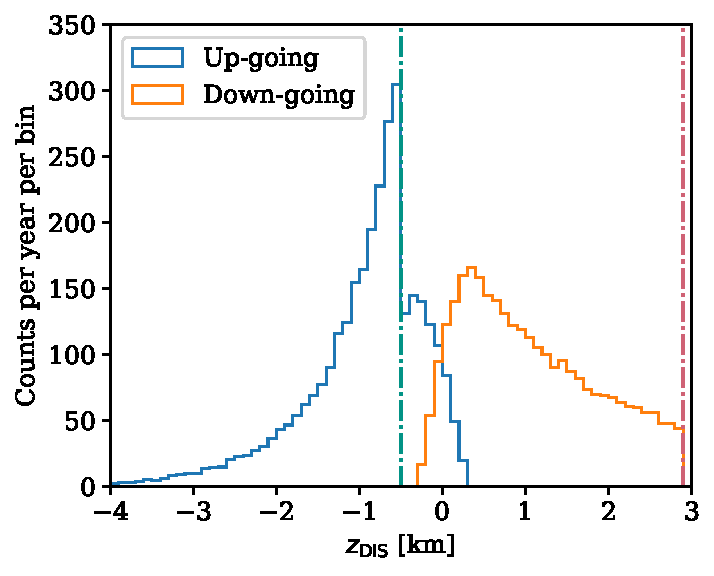
\includegraphics[width=0.75\textwidth]{img/sampling_dis_position.pdf}
    \caption{向上运动和向下运动的事件各自的DIS反应顶点在探测器坐标系下的$z$坐标$z_\mathrm{DIS}$上的分布。其中,绿色的点虚线表示海水与岩层的分界线,红色的点虚线表示海水与空气的分界线。}
    \label{fig:sampling_dis_position}
\end{figure}


\begin{figure}[!htb]%
    \centering
    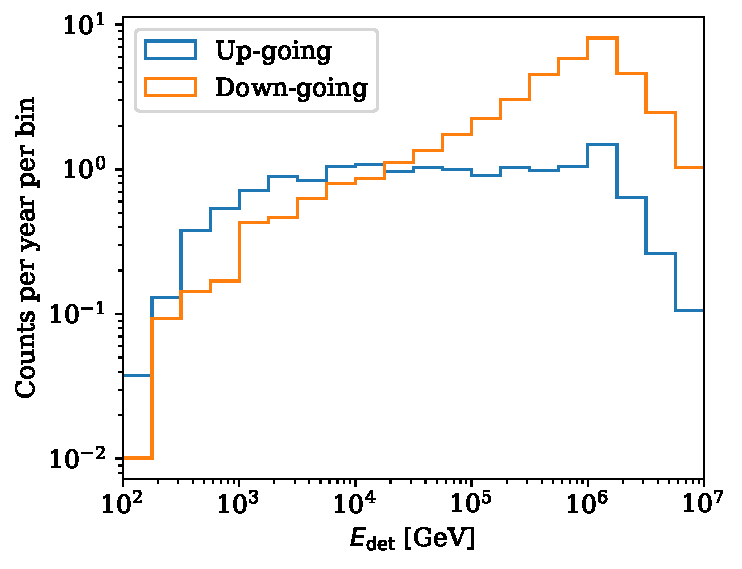
\includegraphics[width=0.75\textwidth]{img/sampling_energy_spectrum_det.pdf}
    \caption{在选取了$E_\nu > 1\,\mathrm{PeV}$的事件之后,向上运动和向下运动的事件到达探测器的能量的分布图。}
    \label{fig:sampling_energy_spectrum_det}
\end{figure}

图\ref{fig:sampling_zenith}展示了不同能量的中微子事件在入射的天顶角$\theta_z$空间下的分布情况。我们可以看到,除了上文中提到的上下几何不对称以外,在能量比较低($E_\nu < 100\,\mathrm{TeV}$)的情况下,水平方向的中微子事件要明显少于其他方向上的事件。这是因为我们的探测器构造像是薄饼状:在水平方向上延展比较宽,半径达到$2\,\mathrm{km}$,而在垂直方向上高度比较小,仅为$0.6\,\mathrm{km}$。这导致了我们探测器接对来自水平方向的事件的有效面积相比于垂直方向有所降低。

\begin{figure}[!htb]%
    \centering
    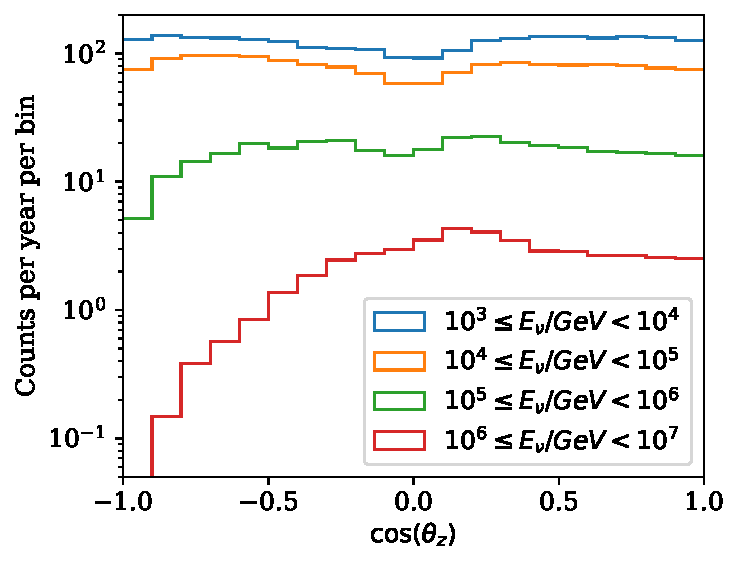
\includegraphics[width=0.75\textwidth]{img/sampling_zenith.pdf}
    \caption{不同能量的中微子事件在入射天顶角空间下的分布。}
    \label{fig:sampling_zenith}
\end{figure}

\subsection{有效面积计算}

在介绍完蒙特卡洛采样中有关采样和事件权重的内容之后,我们可以回到一开始的有效面积计算公式\ref{eq:eff_area_init}中。公式中的$\frac{\mathrm{d}N}{\mathrm{d}t ~\mathrm{d}\Omega ~\mathrm{d}E}(E, \hat{n})$项可以通过将公式\ref{eq:sampling_trigger_rate}微分化得到,而微分操作对应到蒙特卡洛方法中便是对样本进行分区间计算:
\begin{equation}
    \frac{\mathrm{d}N}{\mathrm{d}t \mathrm{d}E \mathrm{d}\Omega} = 
    \frac{1}{N_\mathrm{tot} \Delta E \Delta\Omega} \sum_{i \in \mathrm{bin}} \left[ 
    \mathrm{I}_\mathrm{sel}(s_i) \times 
    F_\mathrm{phy} (E_i, \hat{n}_i) \times
    w_{\mathrm{tot}, i} \right] ,
\label{eq:sampling_trigger_rate_diff}
\end{equation}
其中$\sum_{i \in \mathrm{bin}}$表示对属于该能量和立体角范围区间内的事件进行求和,$\Delta E \Delta\Omega$表示区间的相空间大小。

将公式\ref{eq:sampling_trigger_rate_diff}代入到公式\ref{eq:eff_area_init}中可以得到:
\begin{equation}
    A_\mathrm{eff} (\hat{n}, E) = \frac{1}{N_\mathrm{tot} \Delta E \Delta\Omega} \sum_{i \in \mathrm{bin}} \left[ 
    \mathrm{I}_\mathrm{sel}(s_i) \times 
    w_{\mathrm{tot}, i} \right] ,
    \label{eq:eff_area}
\end{equation}
这里,我们已经成功地从有效面积的表达式中约去了中微子源的物理流量$F_\mathrm{phy} (E, \hat{n})$。我们可以看到$A_\mathrm{eff} (\hat{n}, E)$与具体的中微子流量无关,而与探测器的对事件的探测能力$\mathrm{I}_\mathrm{sel}(s_i)$以及中微子的物理性质$w_{\mathrm{tot}, i}$有关,它反应的是探测器对某一种事件类型的探测能力。

通过模拟,我们得到探测器的有效面积与中微子的能量$E_\nu$和入射天顶角$\theta_z$之间的关系如图\ref{fig:eff_area}中所示。
在将$\theta_z$分为向上入射($-1 \leq \theta_z < -0.5$),水平入射($-0.5 \leq \theta_z < 0.5$)和向下入射之后($0.5 \leq \theta_z < 1$)之后,我们对不同入射角区间的有效面积求平均,可以得到图\ref{fig:eff_area_band}中所示的结果。

从图\ref{fig:eff_area_band}中我们可以观察到,对于水平和向下入射的中微子而言,当中微子能量达到$10\,\mathrm{PeV}$时,海铃中微子望远镜的有效面积可以达到$5 \times 10^3\,\mathrm{m^2}$,是IceCube的5倍多\cite{IceCube_10yr_point_source:2019}。
对于向上入射的中微子而言,当中微子的能量达到$100\,\mathrm{GeV}$时,有效面积达到顶峰,约为$10^3\,\mathrm{m^2}$。当能量继续升高时,地球的吸收效应导致有效面积逐渐降低,在$10\,\mathrm{PeV}$时约为$10^2\,\mathrm{m}^2$。

\begin{figure}[!htb]%
    \centering
    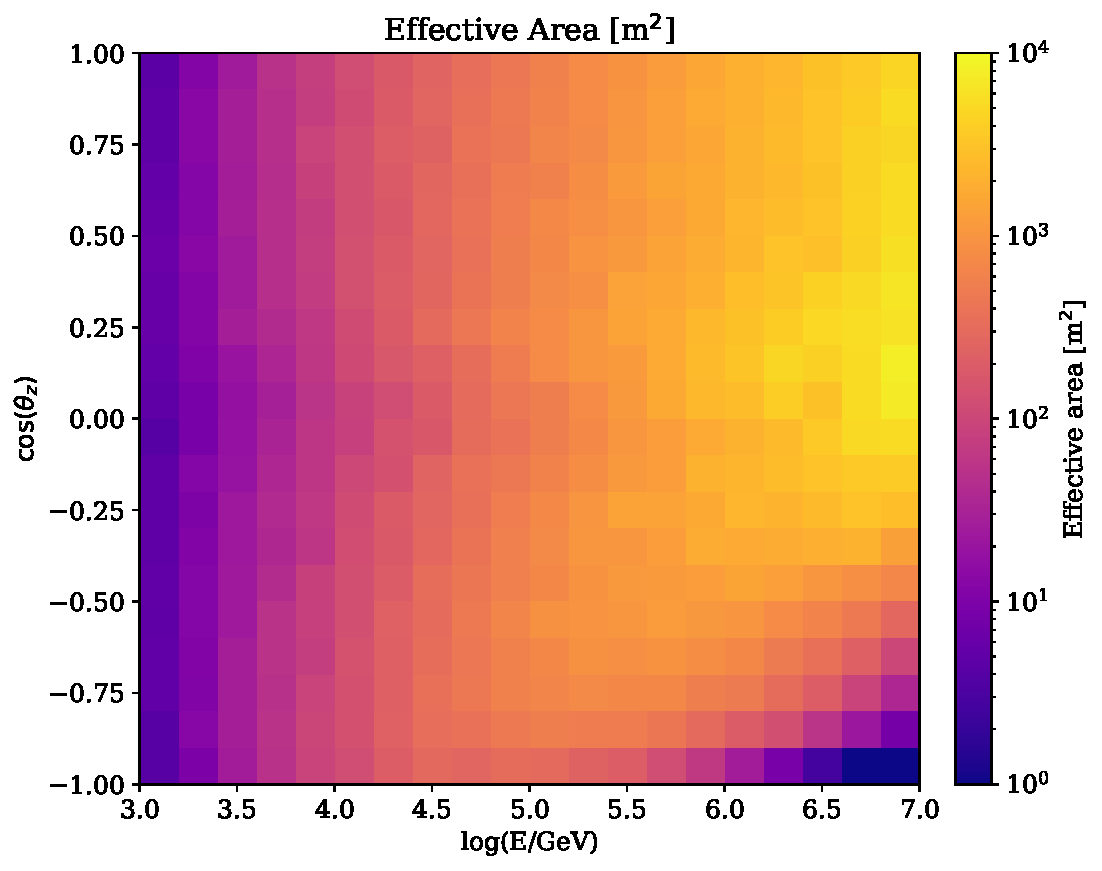
\includegraphics[width=0.90\textwidth]{img/eff_area.pdf}
    \caption{探测器的有效面积与入射中微子的能量以及天顶角之间的关系。}
    \label{fig:eff_area}
\end{figure}

\begin{figure}[!htb]%
    \centering
    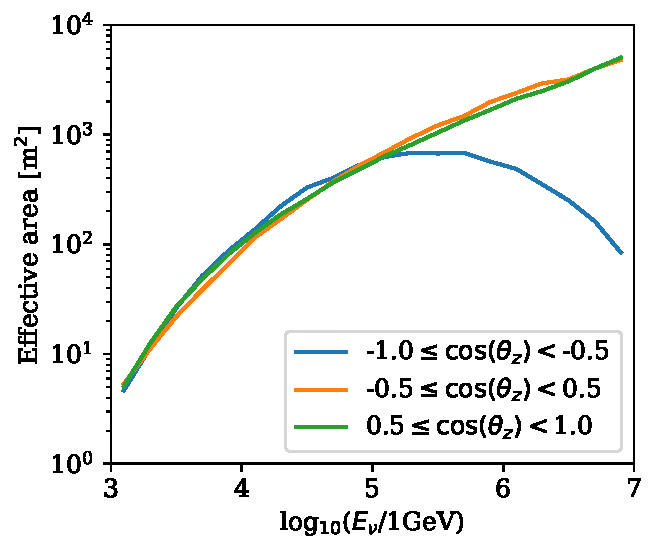
\includegraphics[width=0.65\textwidth]{img/eff_area_band.pdf}
    \caption{不同入射的天顶角下,探测器的有效面积与入射中微子能量的关系。}
    \label{fig:eff_area_band}
\end{figure}

\section{对中微子源的灵敏度}

有了探测器的角度分辨率和有效面积之后,我们便可以开始计算探测器对中微子源的灵敏度。在本章节的灵敏度分析中,我们通过来自地球方向,向上穿行的径迹型事件来寻找中微子的源,即要求天顶角$\theta_z > 85^\circ$,选择这样的事件通道是为了避免数量众多的大气缪子本底的影响。

\subsection{天体源赤纬的影响}

由于探测器的有效面积是与中微子的入射角相关的,因此我们要首先讨论一下来自某一个天体物理中微子源的流量相对于探测器的入射角。
与IceCube那样位于南极点的探测器不同,海铃所处的纬度位置为$16^\circ 8' \mathrm{N}$,因此,它会随着地球的自转而转动。
在海铃看来,宇宙中固定位置的天体物理源在不同的时刻对应的天顶角是不同的:
\begin{equation}
\begin{aligned}
    \cos\theta_z(t) &= \hat{n}_s \, \cdot \, \hat{n}_\mathrm{det}(t) \\
    \hat{n}_\mathrm{det}(t) &= \left(\cos(l_\mathrm{det})\cos(\frac{2\pi t}{T}),\,
    \cos(l_\mathrm{det})\sin(\frac{2\pi t}{T}),\, 
    \sin(l_\mathrm{det}) \right) ,
\end{aligned}
\end{equation}
其中$\hat{n}_s$是该天体物理源在赤道坐标系中的方位,$\hat{n}_\mathrm{det}(t)$表示探测器在赤道坐标系中的方位,它会随着地球的转动而变化。
$l_\mathrm{det}$表示探测器的纬度,$t$表示时间,$T$表示地球的自转周期,即一天。

在各个赤纬天区中,典型的高能天体物理源相对于海铃的入射角随时间的变化曲线$\cos\theta_z(t)$如图\ref{fig:source_zenith_time_curve}所示。
在地球自转一圈的时间中,来自不同赤纬上的天体物理源可以被海铃所观测的时间占总事件的比例如图\ref{fig:source_zenith_duty_cycle}中所示。
从图中可以发现,除了北极点附近赤纬范围内的少数区域外,海铃对大多数天体中微子源都能有较长的观测时间窗口。

\begin{figure}[!htb]%
    \centering
    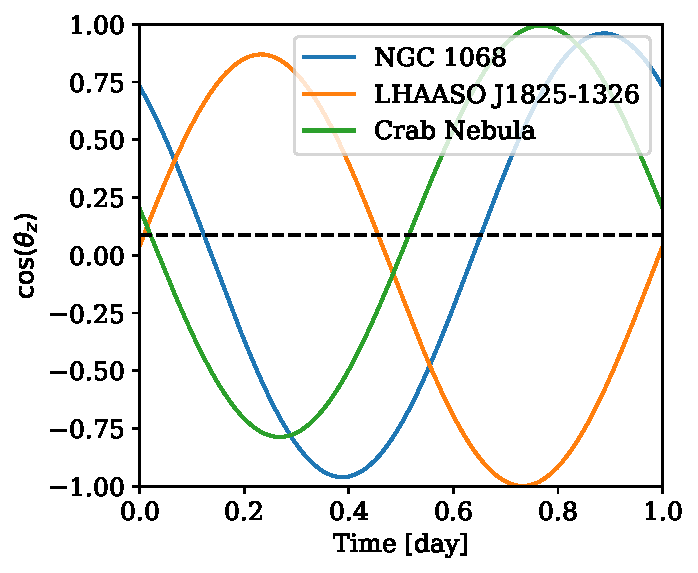
\includegraphics[width=0.60\textwidth]{img/source_zenith_time_curve.pdf}
    \caption{几个潜在的天体物理源在海铃中微子望远镜视角的天顶角随时间的变化。图中选取了北天,赤道和南天各3个源,它们在赤道坐标系下的坐标分别为:NGC 1068:$(\mathrm{02^h 42^m, 00^\circ 00′})$,LHAASO 1825-1326:$(\mathrm{18^h 25^m, -13^\circ 26′})$,Crab:$(\mathrm{05^h 34^m, +22^\circ 00'})$}
    \label{fig:source_zenith_time_curve}
\end{figure}

\begin{figure}[!htb]%
    \centering
    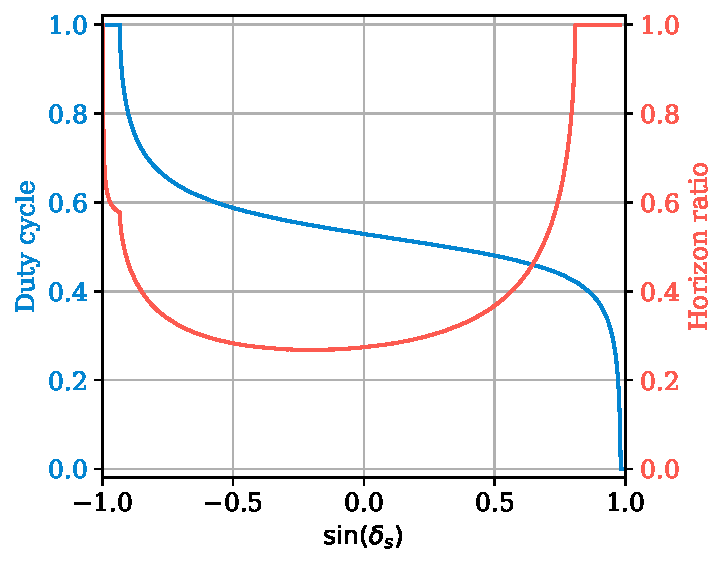
\includegraphics[width=0.60\textwidth]{img/source_zenith_duty_cycle.pdf}
    \caption{海铃中微子望远镜对不同赤纬的天体物理源的可观测时间占比(蓝线)以及在可观测时间中,水平方向的占比(红线)。其中我们将水平方向定义成$100^\circ<= \theta_z <85^\circ$。图中横坐标表示天体物理源的赤纬的正弦值。}
    \label{fig:source_zenith_duty_cycle}
\end{figure}

在图\ref{fig:eff_area}中,我们的有效面积是以探测器为中心的,其横轴表示中微子事件相对于探测器的天顶角。现在,我们以中微子源为考虑对象,定义探测器对不同赤纬的中微子源的有效面积$A_\mathrm{eff}^s$:
\begin{equation}
    A_\mathrm{eff}^s(E_\nu, \delta_s) = \frac{1}{T} \int_0^T A_\mathrm{eff}(E_\nu, \theta_z(t)) \times \mathrm{I}_\mathrm{up}(\theta_z(t)) \, \mathrm{d} t \,   ,
\end{equation}
其中,积分范围$T$表示一天,$\mathrm{I}_\mathrm{up}(\theta_z(t))$表示筛选向上穿行的缪子事件。
这种有效面积的计算方式考虑了该天体物理源在一天的时间内相对于探测器的天顶角的平均效应。

海铃对向上穿行的事件的有效面积如图\ref{fig:eff_area_with_lat}中所示。
可以可以看到,相比于图\ref{fig:eff_area},相对于源的有效面积整体降低了约一半,这是因为探测器的平均可观测时间占比变成了约50\%。
并且在高能处,探测器的有效面积降低得尤其明显,这是因为我们要求中微子事件是向上穿行的,而高能的中微子事件在向上穿行的过程中会经历强烈的地球吸收作用。
而且赤纬范围在$-0.7 < \sin(\delta_s) < 0.7$范围内的源在高能段衰减地比其他赤纬范围要更加明显,这是因为如图\ref{fig:source_zenith_duty_cycle}中所示,在它们的可观测时间中,水平入射的占比很少。
探测器对北极附近的源会有更弱的有效面积,而对于南极的附近的源会有更好的有效面积,与图\ref{fig:source_zenith_duty_cycle}中的探测器可观测时间占比一致。

\begin{figure}[!htb]%
    \centering
    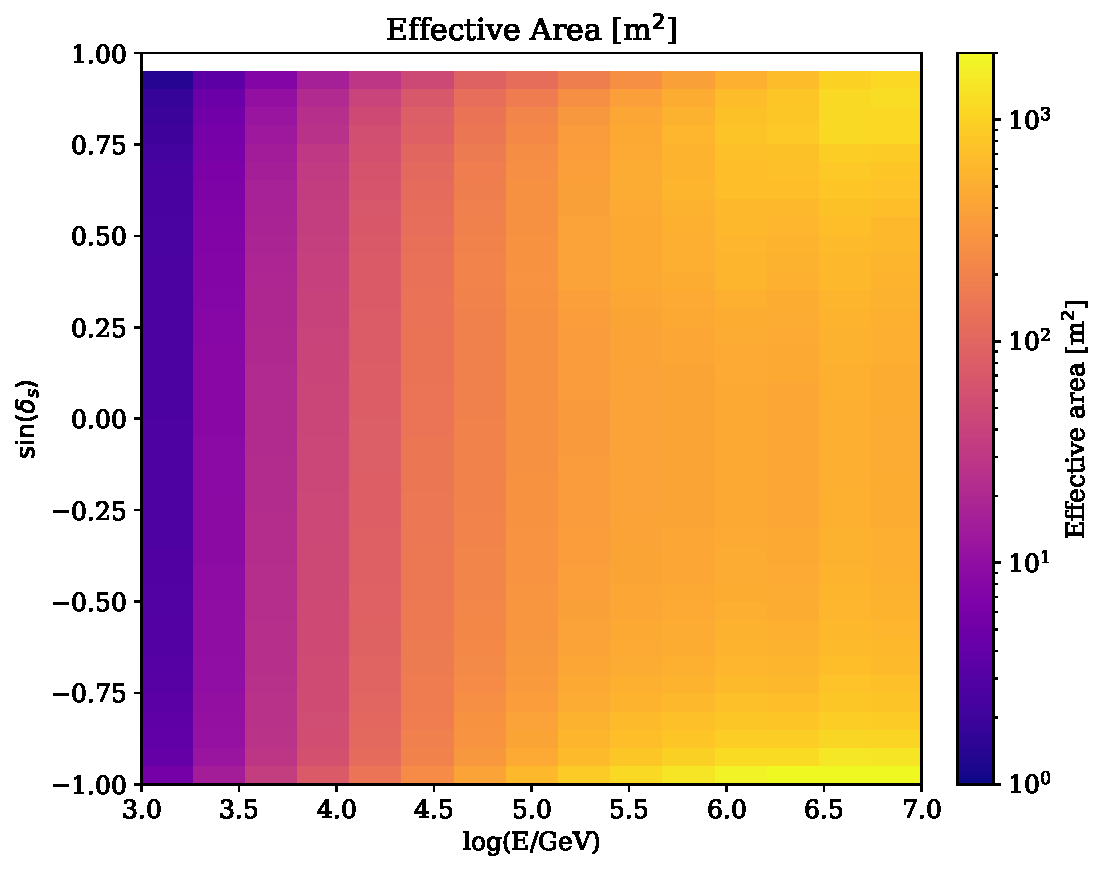
\includegraphics[width=0.80\textwidth]{img/eff_area_with_lat.pdf}
    \caption{海铃中微子望远镜对不同赤纬的天体物理源的有效面积,图中横坐标表示赤纬的正弦值。}
    \label{fig:eff_area_with_lat}
\end{figure}



\subsection{对NGC 1068的显著性}

对于某一假定的中微子天体物理源,我们可以通过分析来自该源的中微子事件在立体角空间上相对于背景事件的超出来计算望远镜对它观测的显著性。
以NGC 1068这个IceCube列表中最有可能的源为例,我们假设源的流强$F_\mathrm{NGC}(E_\nu)$为IceCube的最佳拟合结果\cite{IceCube_NGC1068:2022}。
我们分析中的背景主要包括弥散的中微子辐射背景$F_\mathrm{diff}(E_\nu)$和大气中微子背景$F_\mathrm{atm}(E_\nu)$。
对于这两种背景的流强以及不确定性,我们分别参考了IceCube对弥散缪子中微子流强的观测\cite{IceCube_diffse_muon:2021}和大气中微子的观测\cite{IceCube_atmos_nu:2014}。
上述信号和背景的中微子流强的能谱如图\ref{fig:source_background_flux}中所示。

\begin{figure}[!htb]%
    \centering
    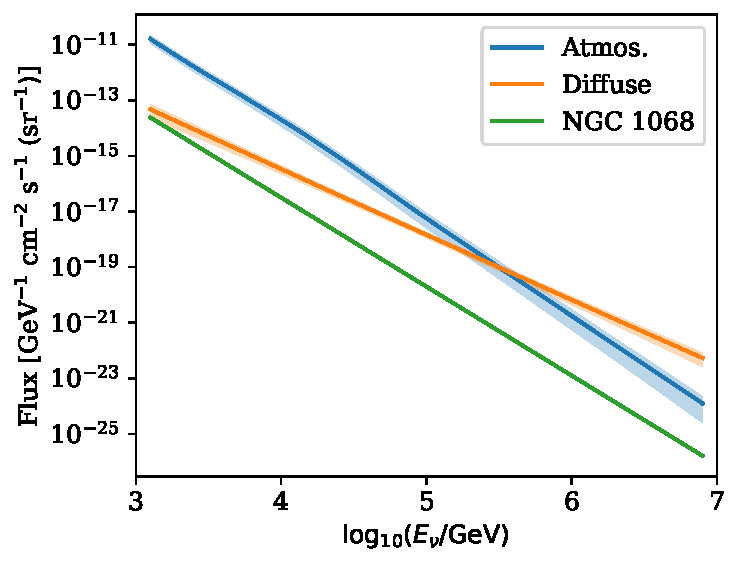
\includegraphics[width=0.70\textwidth]{img/source_background_flux.pdf}
    \caption{IceCube测得的NGC 1068的中微子的流强,弥散天体物理中微子的流强,以及大气中微子的流强,阴影区域表示背景流强的不确定性。注意,图中NGC 1068源是一个点源,其流强单位为$\mathrm{GeV^{-1} cm^{-2} s^{-1}}$,而弥散天体物理中微子和大气中微子流强的单位中包含每立体角,为$\mathrm{GeV^{-1} cm^{-2} s^{-1} sr^{-1}}$。}
    \label{fig:source_background_flux}
\end{figure}

将中微子源流强的能谱与探测器的有效面积做卷积,可以得到探测器探测到的事例率:
\begin{equation}
\begin{aligned}
    \frac{\mathrm{d}N_s}{\mathrm{d}t} &= \int F_s(E_\nu)  A_\mathrm{eff}^s (E_\nu, \delta_s) \,\mathrm{d} E_\nu \\ 
    \frac{\mathrm{d}N_\mathrm{b}}{\mathrm{d}t} &= \Delta \Omega \int F_\mathrm{b}(E_\nu)  A_\mathrm{eff}^s (E_\nu, \delta_s) \,\mathrm{d} E_\nu, \\
\end{aligned}
    \label{eq:event_rate_using_eff}
\end{equation}
其中的$F_s(E_\nu)$表示天体物理源的中微子流量,其量纲为单位时间单位面积的事件数量,注意量纲中不含有立体角。
而对于弥散的中微子流强$F_b(E_\nu)$,由于其流强量纲中含有立体角,因此在计算实例率时需要再乘以$\Delta\Omega$,用于表示对某一中微子天体源中分析时所选取的立体角空间范围。
注意,为了将信号事件全部包含在内,$\Delta\Omega$应当大于探测器的角分辨率。

我们选取观测的半张角的余弦变化值$\Delta\cos\theta_s$为$5\times 10^{-4}$时的角度为观测区域,其对应的半张角为$1.81^\circ$。
在该区域中,我们以$1\,\mathrm{TeV}$为中微子流强能谱作低能截断,模拟中微子望远镜对来自点源的中微子事件的响应。
我们以一年为曝光时间来计算在选取的半张角区域内信号和背景事件的事例率的期望值,其结果如图\ref{fig:event_rate_around_source}中下图所示。
我们可以看到由于中微子信号来自于一个点源,因此方向重建得到的信号事件的角度分布主要集中在0附近,它的扩展反应的是探测器的角度分辨率。
而弥散的背景中微子的方向在点源附近的立体角空间内是均匀分布的,因此经过重建之后在$\Delta\cos\theta_s$相空间中的分布也是均匀的。
我们可以看到,在当前的信号和背景流强假设下,我们对NGC-1068的方向上能够观测到明显的事例率超出。

值得注意的是,我们在本次灵敏度分析时只在中微子方向的相空间中寻找信号超出,而没有考虑中微子能量的相空间,这是因为目前我们还没有完成对径迹型事件的能量重建工作。
对于中微子的能量,我们只用它设置的信号和背景选取的能量阈值,能量阈值的选取对分析结果会有重要的影响,这会在后续内容会有更多的讨论。

\begin{figure}[!htb]%
    \centering
    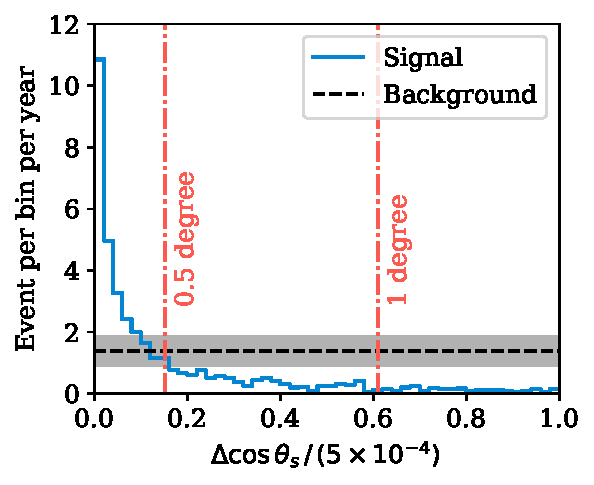
\includegraphics[width=0.70\textwidth]{img/event_rate_around_source.pdf}
    \caption{在$\Delta\cos\theta_s$属于0到$5\times 10^{-4}$的张角范围内,中微子信号和背景事件在方向空间中的事例率的对比。其中信号中微子是来自于NGC 1068源,其能谱指数假设为-3.2。背景中微子是来自于大气中微子和弥散高能中微子。}
    \label{fig:event_rate_around_source}
\end{figure}

接下来,我们来计算该事例率和立体角的分布下,中微子望远镜对NGC 1068源的显著性是多少。
在计算中,我们采用了分区间的似然估计(binned likelihood analysis):
\begin{equation}
\begin{aligned}
    \mathcal{L}(n_s, n_b;\mu, \vec{n}) &=  
    \prod^N_{i=1} \frac{(\mu n_s p_i^s + \mu n_b p_i^b)^{n_i}}{n_i!} 
    e^{-(\mu n_s p_i^s + \mu n_b p_i^b)}
    \times \frac{1}{\sqrt{2\pi}\sigma_b} e^{-\frac{(n_b-n_b^0)^2}{2\sigma_b^2}} \\
    \ln{\mathcal{L}}(n_s, n_b;\mu, \vec{n}) &= 
    -\mu(n_s+n_b) + \sum^N_{i=1} n_i \ln (\mu n_s p_i^s + \mu n_b p_i^b) 
    - \frac{(n_b-n_b^0)^2}{2\sigma_b^2} + C ,
    \label{eq:binned_likelihood}
\end{aligned}
\end{equation}
公式中的第一部分表示每一个区间内的泊松涨落,其中$n_s$和$n_b$表示信号和背景事件的总事例率,在我们的应用中,$n_s$和$n_b$分别表示NGC 1068的事例率和大气中微子以及弥散中微子在$\Delta\cos\theta_s < 5\times 10^{-4}$范围内的总事例率。
$\mu$表示观测的时间,公式中出现的$\mu n_s$和$\mu n_b$表示在观测时间$\mu$下,探测到的总的信号和背景的事件数的期望值。
$n_i$表示观测到的第$i$个区间内的事件数量,$p_i^s$,$p_i^b$分别表示模型中信号和背景在第$i$个区间内的分布概率,在我们的应用中,信号的分布表征着中微子望远镜的角分辨率,而背景是弥散的均匀分布的。$N$是区间的总数。
公式中的第二部分表示对背景事例率偏离模型预测值的惩罚,其中$n_b^0$和$\sigma_b$分别表示我们的模型中对背景事例率的期望和涨落,在我们的应用中,表示IceCube对大气中微子和弥散中微子的测量值和误差。

在对信号的显著性分析中,我们探究一个观测到的信号有多少的可能性是由背景涨落导致的。
在这种情况下,我们假设既观测到了信号又观测到了背景,那么观测到的数据在每一个区间中都应该服从期望为$\mu(n_s p_i^s +  n_b^0 p_i^b)$的柏松分布。
在具体操作中,我们使用了Asimov近似\cite{Cowan_Asimov_estimate:2010},即使用了观测值的期望来代替原本应当是随机分布的观测值:
\begin{equation}
    n_i = \mu(n_s p_i^s +  n_b^0 p_i^b) ,
    \label{eq:asimov_est_signal}
\end{equation}
这样可以避免繁琐的模拟抽样过程,适合在预研阶段对显著性进行快速的估计。

我们研究这样的观测信号有多少可能性是由纯背景所贡献的,因此我们定义如下的检验统计量(test statistics,TS):
\begin{equation}
    \mathrm{TS}(\mu) = 2 \ln \left( \frac
    {\mathcal{L}(\mu n_s, \mu n_b^0; \vec{n})} 
    {\mathcal{L}(0, \mu \hat{n}_b; \vec{n})} \right) ,
    \label{eq:ts_significance}
\end{equation}
其中$\mathrm{TS}(\mu)$表示观测时间$\mu$下的TS值,$\hat{n}_b$表示使得$\mathcal{L}(0, \mu n_b; \vec{n})$达到最大的背景事例率。

这样定义的TS中,只有$n_b$这一个自由参数被最大化了,因此TS应当服从自由度为1的卡方分布\cite{Cowan:1998}:
\begin{equation}
    \mathrm{TS} \sim \chi^2(1)
\end{equation}
代入公式\ref{eq:asimov_est_signal}中Asimov近似下观测的事件数的期望,可以得到TS值,并且我们可以根据卡方检验中的概率分布来得到该TS值对应到标准高斯分布$\mathcal{N}(x)$中的显著性$\sigma$:
\begin{equation}
    \int^\infty_\mathrm{TS} \chi^2(x, 1) \mathrm{d}x = 
    2 \int^\infty_\sigma \mathcal{N}(x) \mathrm{d}x ,
    \label{eq:ts_to_sigma}
\end{equation}

最终计算到显著性关于观测时间的函数$\sigma(\mu)$如图\ref{fig:ngc_significance_time_curve}中所示。
在图中,我们绘制了几条不同能量筛选阈值下显著性结果,可以看到在$1\,\mathrm{TeV}$和$3.2\,\mathrm{TeV}$的能量阈值下,海铃可以在约0.5年的观测时间内就以$5\sigma$的置信度发现NGC 1068这个源。
而如果能量阈值选取到$10\,\mathrm{TeV}$,则需要约1.5年的时间才可以达到$5\sigma$。
这是由于NGC 1068源的谱指数为-3.2,比弥散的高能中微子流更软,它的主要中微子信号都集中在$1\,\mathrm{TeV}$到$10\,\mathrm{TeV}$能段。
从图\ref{fig:event_rate_around_source_energy_threshold}中可以看到,当能量阈值取到$10\,\mathrm{TeV}$时,总事例率将降低到约4个事件每年,尽管此时背景事例率非常稀少,但在如此低的事例率下仍然难以实现高置信度。

如果我们在分析中加入对中微子能量重建的不确定度,在这个能段径迹型缪子中微子的能量重建的不确定度在对数空间中大约有0.5到1个量级左右。加入能量重建在一方面将会使我们上述分析中的能量阈值出现一定的波动,造成信号的显著性降低。
而另一方面,加入中微子能量的分析可以使我们做信号关联的相空间从单个立体角的维度扩充到立体角加上能量的维度,这可以在一定程度上提高信号显著性。
因此我们可以合理地推测,即便考虑了能量重建的影响,海铃仍然能够在$\lesssim 1$年的时间内以$5\sigma$的置信度发现NGC 1068这个源。

\begin{figure}[!htb]%
    \centering
    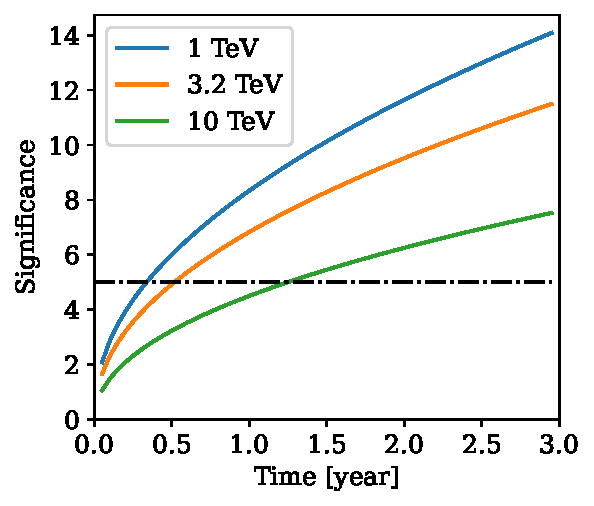
\includegraphics[width=0.55\textwidth]{img/ngc_significance_time_curve.pdf}
    \caption{海铃中微子望远镜观测到NGC 1068源在不同的中微子能量阈值截断下的显著性随时间变化的曲线。}
    \label{fig:ngc_significance_time_curve}
\end{figure}

\subsection{全天中微子源的灵敏度与显著性分析}

在本小节中,我们探讨海铃对来自全天的各个方向的源的灵敏度。我们将望远镜的观测时间固定为10年,假设天体物理源辐射中微子的能谱指数为-2并选取$40\,\mathrm{TeV}$来作为事件筛选的能量阈值,观察对于来自各个不同赤纬的源而言,其流量需要达到多少才能满足以$5\sigma$的置信度发现源的信号的要求。
我们将$5\sigma$发现流量阈值与源的赤纬的曲线称为望远镜的$5\sigma$显著性曲线,其分析结果如图\ref{fig:all_sky_sensitivity_E2}中的红色实线所示,图中同样展示了其他望远镜的$5\sigma$显著性曲线。
可以看到在南天区($\sin(\delta)<0$),海铃的的$5\sigma$显著性曲线相较于IceCube要低约两个量级,在北天区($\sin(\delta)>0$),海铃也比IceCube要低5-6倍。

而如果我们将源的能谱指数改成更软的$-3$能谱,并且选取$1\,\mathrm{TeV}$来作为事件筛选的能量阈值,分析得到$5\sigma$显著性曲线将如图\ref{fig:all_sky_sensitivity_E2}中所示。

\begin{figure}[!htb]%
    \centering
    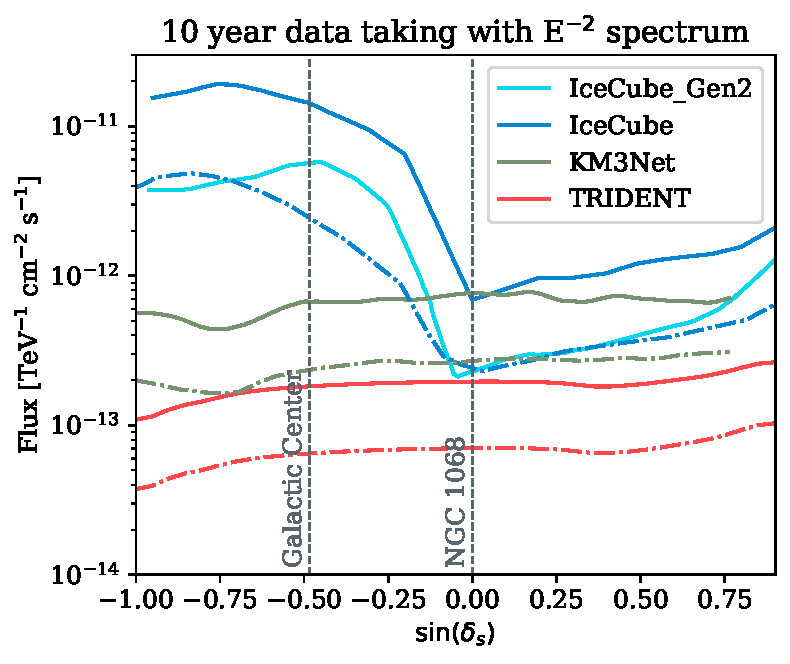
\includegraphics[width=0.65\textwidth]{img/all_sky_sensitivity_E2.pdf}
    \caption{海铃探测器10年数据累积下的全天点源的90\%灵敏度曲线(虚线)和$5\sigma$显著性曲线(实线)。世界上的其他中微子望远镜望远镜:IceCube\cite{IceCube_10yr_point_source:2019},IceCube-Gen2\cite{IceCube-Gen2_sensitivity:2021}和KM3NeT\cite{KM3NeT_sensitivity:2018}的数据也展示了在图中,其中KM3NeT的数据是从6年的观测时间放大到10年的观测时间得到的,假设显著性和灵敏度都随着时间的平方增长。在分析中,我们假设源的能谱指数为-2,对中微子事件筛选的能量阈值为$40\,\mathrm{TeV}$。}
    \label{fig:all_sky_sensitivity_E2}
\end{figure}

\begin{figure}[!htb]%
    \centering
    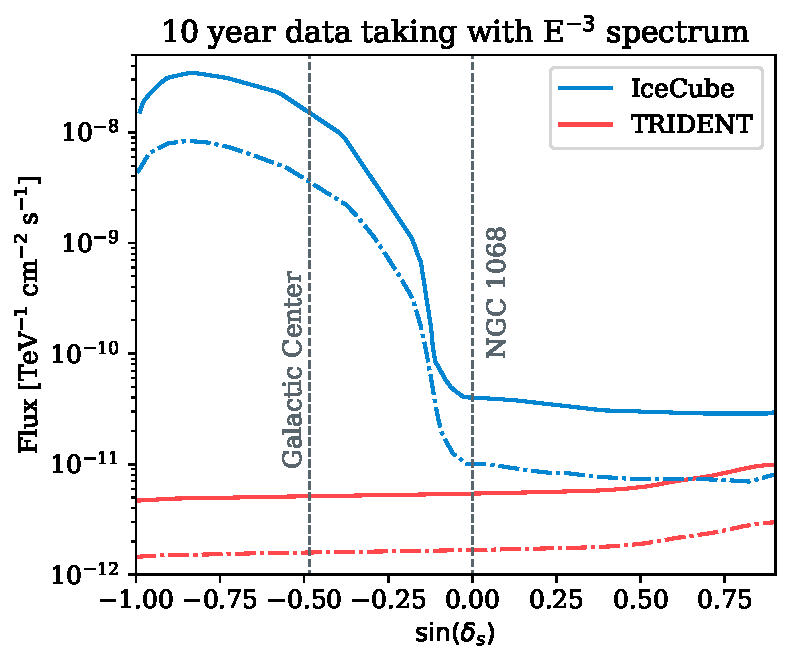
\includegraphics[width=0.65\textwidth]{img/all_sky_sensitivity_E3.pdf}
    \caption{类似于图\ref{fig:all_sky_sensitivity_E2},但是,假设源的能谱指数为-3,对中微子事件筛选的能量阈值为$1\,\mathrm{TeV}$。}
    \label{fig:all_sky_sensitivity_E3}
\end{figure}

除了$5\sigma$显著性曲线以外,衡量探测器寻找天体物理源的另外一个重要属性是90\%灵敏度曲线。
90\%灵敏度表示在纯背景假设下,需要多强的流量才能使得信号能够以90\%的几率超出背景。
通常而言90\%灵敏度曲线对中微子流量的要求会比$5\sigma$显著性曲线要低半个多量级,因为前者表示探测器有可能能发现源的信号超出迹象,而后者要求探测器信号超出要达到非常高($5\sigma$)的显著性。
在分析计算90\%灵敏度时,我们假设只观测到了背景,那么观测到的数据在每一个区间中的数量$\mu(n_b^0 p_i^b)$(使用Asimov近似)。
我们将TS定义为:
\begin{equation}
    \mathrm{TS}(\mu) = 2 \ln \left( \frac
    {\mathcal{L}(0, \mu n_b^0; \vec{n})} 
    {\mathcal{L}(\mu n_s, \mu \hat{n}_b; \vec{n})} \right) ,
    \label{eq:ts_sensitivity}
\end{equation}
其中$\hat{n}_b$表示使得$\mathcal{L}(\mu n_s, \mu n_b; \vec{n})$达到最大的背景事例率。
同样的,$\mathrm{TS}(\mu)$会符合自由度为1的卡方分布,我们寻找能够使得:
\begin{equation}
    \int^\infty_\mathrm{TS} \chi^2(x, 1) \mathrm{d}x = 10\% ,
    \label{eq:ts_to_90}
\end{equation}
的信号事例率,并将之转换为流强,即能够得到90\%灵敏度所对应的信号流强。
对于能谱指数为-2和-3的源,海铃的90\%灵敏度曲线分别如图\ref{fig:all_sky_sensitivity_E2}和图\ref{fig:all_sky_sensitivity_E3}中红色虚线所示。

